\documentclass[12pt,letterpaper,pdftex]{report}
\usepackage{graphicx}
\usepackage{amsmath}
\usepackage{amssymb}
\usepackage{amsfonts}
\usepackage{amsthm}
\usepackage{bm}
\usepackage{paralist}
% \usepackage{sudoku}
\usepackage{booktabs}
\usepackage{url}
\usepackage{xspace}
\usepackage[pdftex,letterpaper,left=1in,top=1in,bottom=1in,right=1in,includeheadfoot]{geometry}
\usepackage{fancyhdr}
\usepackage[shortlabels]{enumitem}
\pagestyle{fancy}
\lhead{\footnotesize Tutorial 4: CS3243 Introduction to AI \\ \bf {Issued: Sep 09, 2019}}
\rhead{\footnotesize Semester 1, AY 2019/20 \\ \bf{Due: Week 6 Tutorial}}
\lfoot{}
\cfoot{}
\rfoot{\thepage}
\renewcommand{\headrulewidth}{1pt}
\usepackage{times}
%\usepackage[boxed]{algorithm}
%\usepackage[noend]{algorithmic}
\usepackage[pdftex]{epsfig}

\usepackage{algorithm}
\usepackage{algcompatible}

\usepackage{comment}
% \specialcomment{solution}{\paragraph{\textbf{Solution:}}}{\par}
%\excludecomment{solution}



\usepackage{tabularx}
\newtheorem{theorem}{Theorem}
\newtheorem{proposition}[theorem]{Proposition}
\newtheorem{lemma}[theorem]{Lemma}
\newtheorem{corollary}[theorem]{Corollary}
\theoremstyle{definition}
\newtheorem{definition}[theorem]{Definition}

\newcommand{\ma}[1]{{\bf #1}}
\newcommand{\ve}[1]{{\mathbf #1}}
\newcommand{\set}[1]{{\mathcal #1}}
\newcommand{\E}{\mathbb{E}}
% The ``defined as'' symbol.
\newcommand{\defeq}[0]{\ensuremath{\stackrel{\triangle}{=}}}
\renewcommand{\cal}[1]{\mathcal{#1}}
\newcommand{\tup}[1]{\langle #1 \rangle}
\newcommand{\true}{\texttt{true}\xspace}
\newcommand{\false}{\texttt{false}\xspace}
\newcommand{\Neighbors}{\mathtt{Neighbors}}

\newcommand{\skipit}[1]{}


\begin{document}

% \begin{center}
% {{\bf National University of Singapore}}\\
% {{\bf School of Computing}}\\
% {{\bf CS3243 Introduction to AI}}\vspace{5mm}\\

% {{\bf Tutorial 1}}\\
% \end{center}
% Issued: \today \hfill Due: Week 3 in the tutorial class
% \hrule\vspace{5mm}
% \noindent
{\bf Instructions}:
\emph{
	\begin{compactitem}
	\item Your solutions for this tutorial must be TYPE-WRITTEN.
	\item Submit your solution(s) to your tutor. You can make another copy for
	yourself if necessary. Late submission will NOT be entertained.
	\item YOUR SOLUTION TO QUESTION $1$ will be GRADED for this tutorial.
	\item You can work in pairs, but each of you should submit the solution(s) individually.
	\item Include the name of your collaborator in your submission.
	\end{compactitem}
}

\vspace{5mm}
% \renewcommand*\sudokuformat[1]{\Large\rmfamily#1}
% \setlength\sudokusize{8cm}

\begin{table}[]
	\begin{tabular}{|l|p{5cm}|l|p{2cm}|}
	  \hline
	  Name         &  & Matric number                &  \\ \hline
	  Collaborator &  & Collaborator's matric number &  \\ \hline
	  Tutorial & \multicolumn{3}{l|}{} \\ \hline
 	\end{tabular}
  \end{table}





\begin{enumerate}
% --------------- Question1 ----------------
\item Prove that $\alpha$-$\beta$ pruning does not remove any strategies that
are played in a Nash equilibrium of an extensive form game; can $\alpha$-$\beta$
pruning be used to find a subgame-perfect Nash equilibrium? Prove or provide a
counterexample. 

\noindent \textbf{Solution:}

\textbf{Your solution here}

    
% --------------- Question2 --------------- 
\item Consider the following game: we have an attacker looking at three targets:
$t_1,t_2$ and $t_3$. A defender must choose which of the two targets it will
guard; however, the attacker has an advantage: it can observe what the defender
is doing before it chooses its move. If an attacker successfully attacks it
receives a payoff of 1 and the defender gets a payoff of $-1$. 
\begin{enumerate}
	\item Model this problem as a minimax search problem. Draw out the search
	tree. What is the defender's payoff in this game?
	\item Can the defender do better by randomizing? What is the defender's
	optimal strategy? Prove your claim. 
\end{enumerate}



\noindent \textbf{Solution:}

\textbf{Your solution here}


% --------------- Question3 --------------- 
\item Assume that we have the following initial state and goal state for the
8-puzzle game.  We will use $h_1$ defined as ``the number of misplaced tiles''
to evaluate each state.
\begin{center}
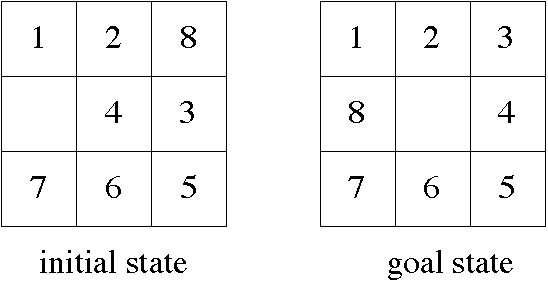
\includegraphics[totalheight=1.5in]{week6images/8puzzle.pdf}
\end{center}
\begin{enumerate}
	\item Apply the hill-climbing search algorithm in Figure~$4.2$ of AIMA $3$rd
	edition. Can the algorithm reach the goal state?
	\item Identify a sequence of actions leading from the initial state to the
	goal state. % Is it possible for simulated annealing to find such a
	solution?
\end{enumerate}



\noindent \textbf{Solution:}

\textbf{Your solution here}



% --------------- Question4 --------------- 


\item Consider the two-player game described in Figure~\ref{fig:definegame}. For example, if $A$ is on $3$ and B is on $2$, then $A$ may move back to $1$. The game ends when one player reaches the opposite end of the board. If
player $A$ reaches space $4$ first, then the value of the game to $A$ is $+1$, if player $B$ reaches
space $1$ first, then the value of the game to A is -1.
\begin{figure}[ht]
	\centering
	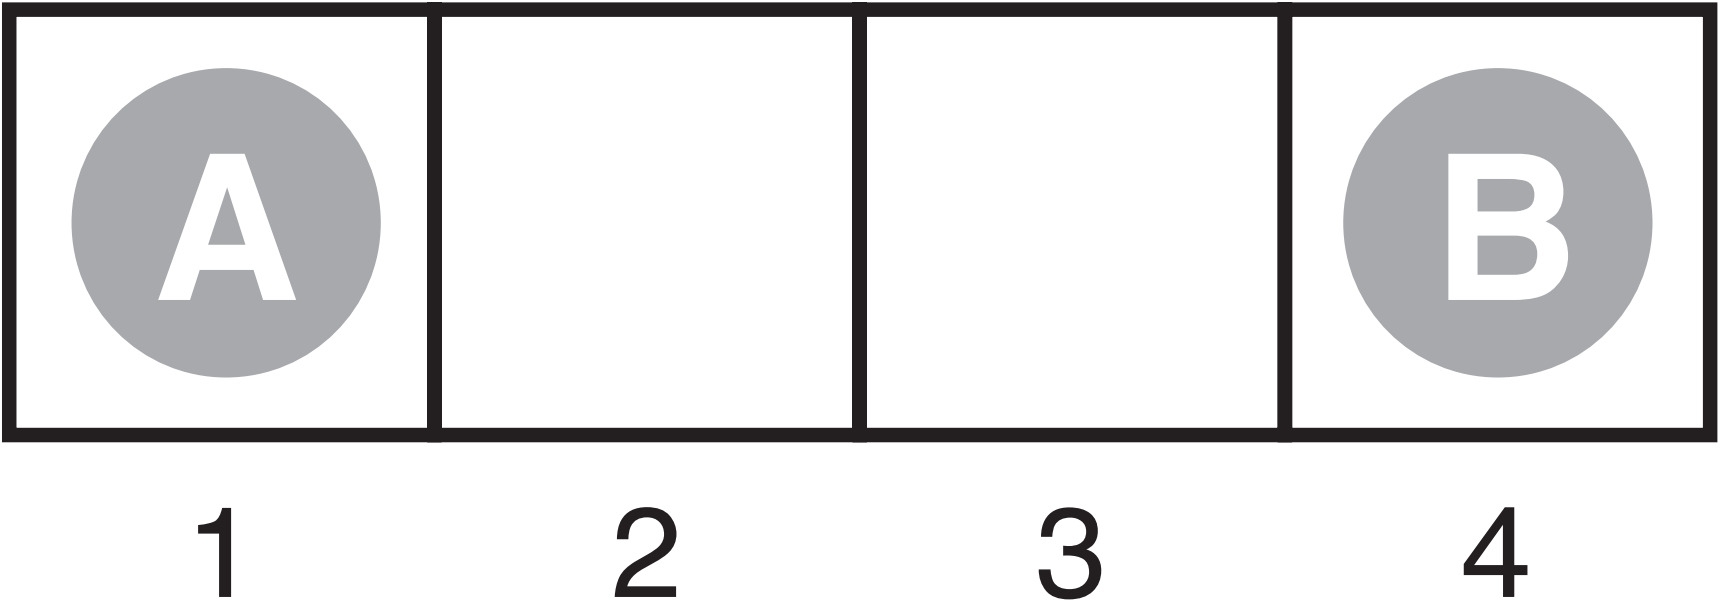
\includegraphics[width=0.5\textwidth]{week6images/defined_game.png}
	\caption{The starting position of a simple game. Player A moves first. The two players take turns moving, and each player must move his token to an open adjacent space in either direction. If the opponent occupies an adjacent space, then a player may jump over the opponent to the next open space if any.}
	\label{fig:definegame}
\end{figure}
\begin{enumerate}
	\item Draw the complete game tree, using the following conventions:
	\begin{itemize}
		\item Write each state as $(s_A, s_B)$, where $s_A$ and $s_B$ denote the token locations.
		\item Put each terminal state in a square box and write its game value in a circle.
		\item Put loop states (states that already appear on the path to the root) in double square
		boxes. Since their value is unclear, annotate each with a “?” in a circle.
	\end{itemize}
	\item Explain why the standard minimax algorithm would fail on this game tree and briefly
	sketch how you might fix it, drawing on your answer to (a). Does your modified algorithm give optimal decisions for all games with loops?
	\item This 4-square game can be generalized to n squares for any $n > 2$. Prove that $A$ wins
	if $n$ is even and loses if $n$ is odd.
\end{enumerate}


\noindent \textbf{Solution:}

\textbf{Your solution here}

% ================= END ================= 
\end{enumerate}
\end{document}
